\documentclass[14pt]{beamer}

\usepackage[english]{babel}

\usepackage[latin1]{inputenc}

\usepackage[T1]{fontenc}

\usepackage{amsmath}
\usepackage{amsfonts}
\usepackage{amssymb}
\usepackage{amsthm}

%\usepackage{tgtermes}
\usepackage{tgheros}
%\usepackage{cmbright}
\usepackage{qtxmath}
%\usepackage{kpfonts}
\renewcommand{\ttdefault}{txtt}

%\usepackage[amsmath,thmmarks]{ntheorem}

\usepackage{graphics}
\usepackage{url}
\usepackage{listings}
\lstset{
  numbers=none,
  basicstyle=\footnotesize\ttfamily,
  xleftmargin=1em,
  xrightmargin=0em,
  aboveskip=1em,
  belowskip=1em
}

\setbeamertemplate{navigation symbols}{}
\setbeamertemplate{headline}{}
\setbeamertemplate{footline}{}
\usetheme{default}
%\usecolortheme[named=red]{structure}


\title{Agile Development\\
  {\small or:}\\
  {\normalsize Modern Practices in Software Development}}

\author{Martijn Vermaat}
\institute{Human Genetics, LUMC}
\date{\small Bioinformatics work discussion, March 8, 2011}


\begin{document}


\frame{\titlepage}


\frame{

  {\bf Discussion} -- {\em what methods do you use?}

  \vspace{\baselineskip}
  \vspace{\baselineskip}

  Please interrupt, don't be quiet.

}


\frame{

  % picture of waterfall
  % http://www.flickr.com/photos/hamed/462658709/
  {\centerline{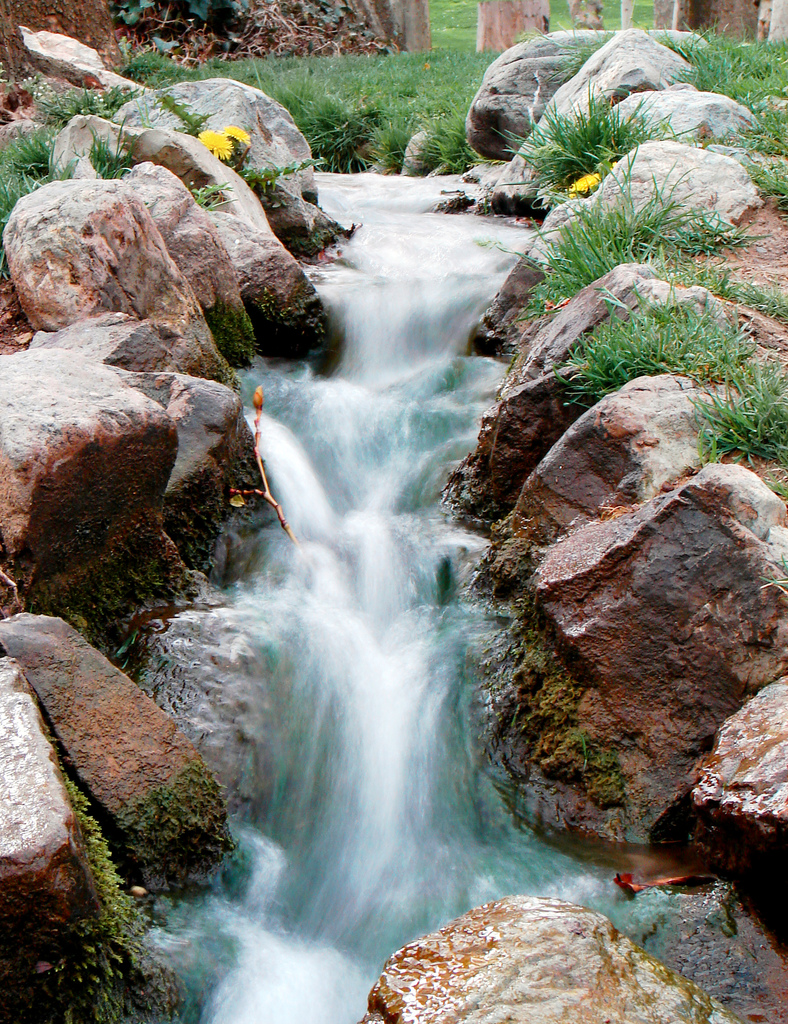
\includegraphics[height=0.8\paperheight,transparent]{images/waterfall.jpg}}}

}


\frame{

  % picture of waterfall model
  % http://www.flickr.com/photos/joomlatools/2283896218/
  {\centerline{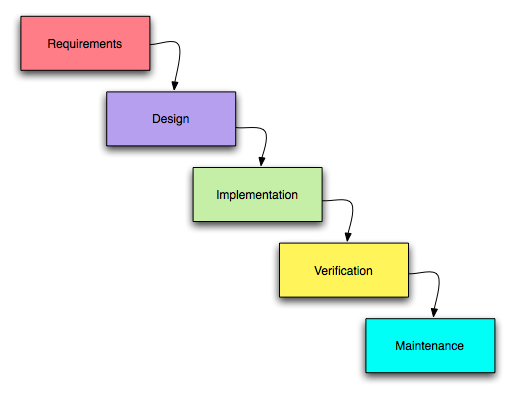
\includegraphics[width=0.8\linewidth,transparent]{images/waterfall-model.png}}}

}


\frame{

  Traditional methods for software development

  \vspace{\baselineskip}

  {\small Waterfall model, spiral model, V-Model, SSADM, \ldots}

  \vspace{\baselineskip}

  \pause

  \begin{itemize}
    \item since 1970s
    \item {\bf heavyweight}
    \item {\bf sequential}
    \item emphasis on r.e. \& design phases
    \item {\bf static}
    \item think large teams
  \end{itemize}

}


\frame{

  % Thick-billed Flowerpecker (Dicaeum agile)
  % http://www.flickr.com/photos/snapflickr/3890553276/
  {\centerline{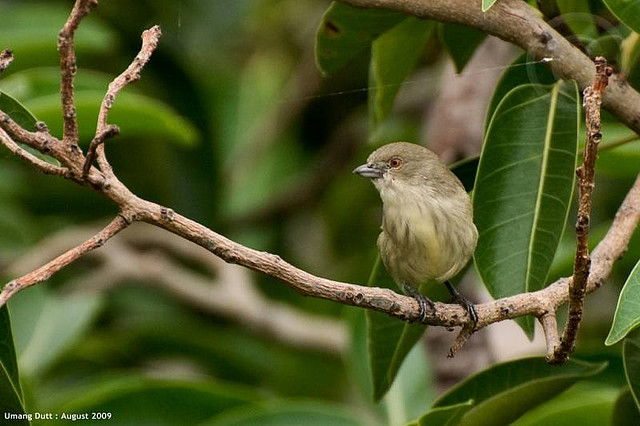
\includegraphics[width=0.8\linewidth,transparent]{images/agile.jpg}}}

}


\frame{

  Agile methods for software development

  \vspace{\baselineskip}

  {\small Extreme Programming, RAD, SCRUM, Agile, \ldots}

  \vspace{\baselineskip}

  \pause

  \begin{itemize}
    \item since mid 1990s
    \item {\bf lightweight}
    \item {\bf iterative and incremental}
    \item emphasis on social interactions
    \item {\bf adapt to changes}
    \item works well for smallish teams ($\leq 10$)
  \end{itemize}

}


\frame{

  Agile development practices

  \vspace{\baselineskip}

  \pause

  \begin{itemize}[<+->]
    \item Test Driven Development\\
      \hspace{8pt} {\small XP, short writing tests $\leftrightarrow$ writing code cycles}
    \item Code review\\
      \hspace{8pt} {\small peer reviewed publishing applied to software}
    \item Continuous Integration\\
      \hspace{8pt} {\small high frequency quality control}
    \item Pair Programming\\
      \hspace{8pt} {\small 2 programmers, 1 work station}
    \item Sprints\\
      \hspace{8pt} {\small short \& intense bursts of programming}
  \end{itemize}

}


\frame{

  {\em Detour}: mechanical checks of simple properties

  \vspace{\baselineskip}

  \begin{itemize}
    \item<2-> {\bf types}: {\em general} but {\em weak} theorems\\
      {\small usually checked statically}
    \item<3-> {\bf contracts}: {\em general} and {\em strong} theorems\\
      {\small checked dynamically for particular instances that occur during regular program operation}
    \item<4-> {\bf unit tests}: {\em specific} and {\em strong} theorems\\
      {\small checked quasi-statically on particular `interesting instances'}
  \end{itemize}

  \vspace{\baselineskip}

  {\small (slide stolen from Benjamin C. Pierce)}

}


\begin{frame}[fragile]

  {\em Example}: merging of lists

  \vspace{\baselineskip}

  Take two sorted lists, and from their elements create a new sorted list.

  \vspace{\baselineskip}

  {\small Example in Python:
  \begin{lstlisting}
>>> l = [1, 3, 6]
>>> r = [2, 3, 5]
>>> merge(l, r)
[1, 2, 3, 3, 5, 6]
  \end{lstlisting}}

\end{frame}


\begin{frame}[fragile]

  {\em Example}: merging and {\bf types}

  \vspace{\baselineskip}

  \pause

  {\small Java, unsafe collections:
  \begin{lstlisting}
public static List merge(List l, List r) { ... }
  \end{lstlisting}}

  \pause

  {\small Java, with generics:
  \begin{lstlisting}
public static <T extends Comparable<? super T>>
              List<T> sort(List<T> l, List<T> r)
  { ... }
  \end{lstlisting}}

  \pause

  {\small Coq, dependently typed vectors:
  \begin{lstlisting}
Fixpoint merge n (l:vector A n) m (r:vector A m) :
  vector A (n+m) := ... .
  \end{lstlisting}}

\end{frame}


\begin{frame}[fragile]

  {\em Example}: merging and {\bf contracts}

  \vspace{\baselineskip}

  \pause

  {\small Java, contracts as comments:
  \begin{lstlisting}
// @param l: a sorted list of elements
// @param r: a sorted list of elements
// @return:  contents of l and r, merged, sorted
public static List merge(List l, List r) { ... }
  \end{lstlisting}}

  \pause

  {\small Java, with Contracts for Java:
  \begin{lstlisting}
@Requires({"Collections.isSorted(l)",
           "Collections.isSorted(r)"})
@Ensures({"Collections.containsSame(
             result, Lists.concatenate(l, r)
           )",
          "Collections.isSorted(result)"})
public static List merge(List l, List r) { ... }
  \end{lstlisting}}

\end{frame}


\begin{frame}[fragile]

  {\em Example}: merging and {\bf unit tests}

  \vspace{\baselineskip}
  \vspace{\baselineskip}

  \pause

  {\small Python:
  \begin{lstlisting}
def merge(l, r):
    ...

def test_merge():
    l = [1, 3, 4, 6]
    r = [1, 2, 5]
    assert merge(l, r) == [1, 1, 2, 3, 4, 5, 6]
  \end{lstlisting}}

\end{frame}


\frame{

  % http://www.flickr.com/photos/thebottomlesspaddlingpool/4767257252
  \begin{center}
    Test Driven Development\\
    \vspace{\baselineskip}
    \vspace{\baselineskip}
    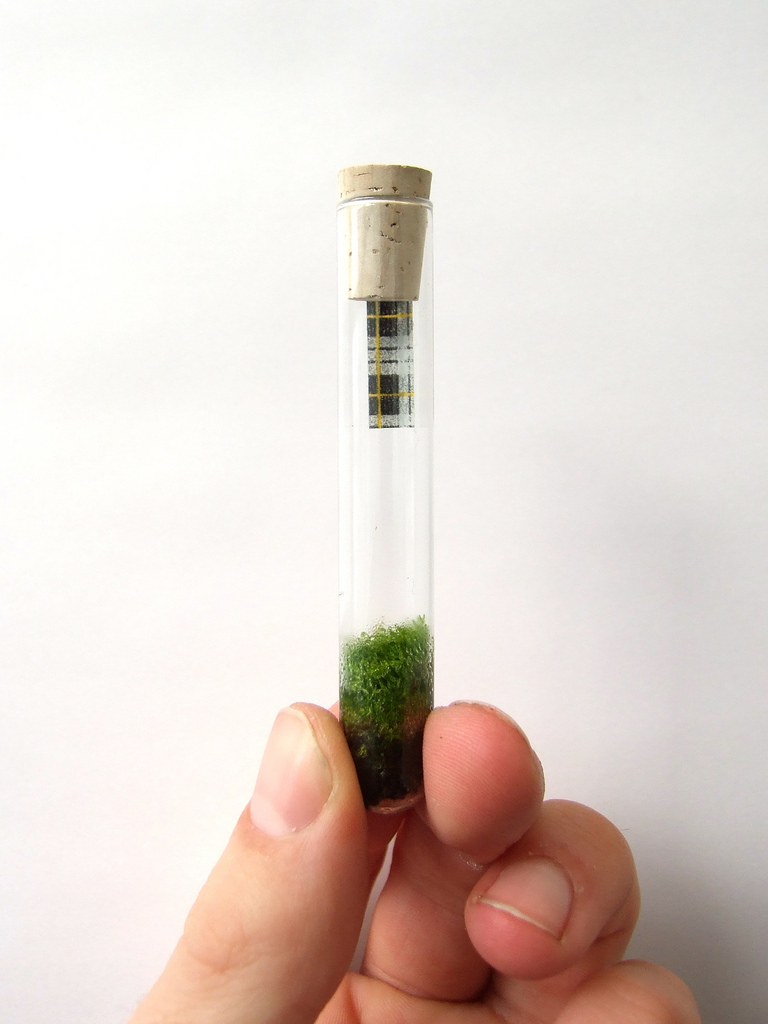
\includegraphics[height=0.6\paperheight,transparent]{images/test.jpg}
  \end{center}

}


\frame{

  Test Driven Development

  \vspace{\baselineskip}

  \pause

  \begin{enumerate}[<+->]
    \item write a test (unit test)
    \item run tests $\rightarrow$ new test fails
    \item write code
    \item run tests $\rightarrow$ on failure, go back
    \item refactor code
    \item repeat
  \end{enumerate}

}


\frame{

  % http://www.flickr.com/photos/carolnichols/2873491547/
  \begin{center}
    Code review\\
    \vspace{\baselineskip}
    \vspace{\baselineskip}
    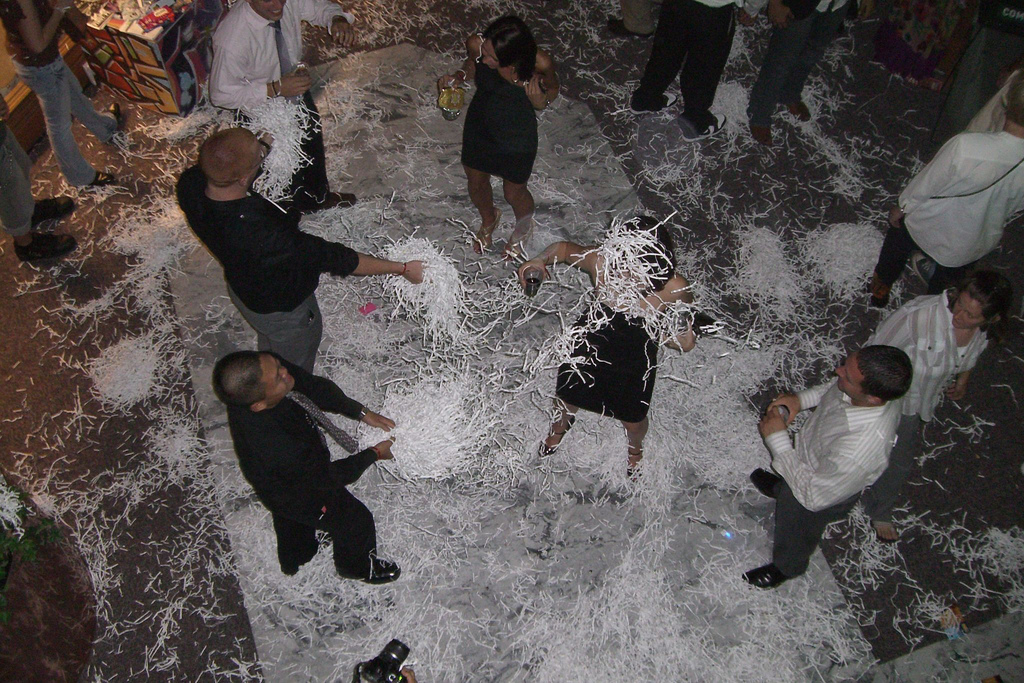
\includegraphics[width=0.6\linewidth,transparent]{images/code-review.jpg}
  \end{center}

}


\frame{

  Code review

  \vspace{\baselineskip}

  \pause

  Spectrum:
  \begin{itemize}
    \item pair programming
    \item informal walkthroughs % Todo: make bold afterwards
    \item formal inspections
  \end{itemize}

  \vspace{\baselineskip}

  \pause

  Compare: peer-reviewed publishing.

  \vspace{\baselineskip}

  \pause

  Common process in Open Source projects:

  \hspace{1cm}{\small pull request $\rightarrow$ review $\leftrightarrow$ change $\rightarrow$ merge}

}


\frame{

  Code review tools

  \vspace{\baselineskip}

  {\small Review Board, Mondrian/Rietveld, Gerrit, Trac plugin, Github, \ldots}

  \vspace{\baselineskip}

  \pause

  Automated code reviewing software
  {\small\begin{itemize}
    \item static code analysis (lint)
    \item visualisation of software structures
  \end{itemize}}

}


\frame{

  % http://www.flickr.com/photos/paldies/85684217/
  \begin{center}
    Continuous Integration
    \vspace{\baselineskip}
    \vspace{\baselineskip}
    
\includegraphics[width=0.6\linewidth,transparent]{images/integration.jpg}
  \end{center}

}


\frame{

  Continuous Integration

  \vspace{\baselineskip}

  \pause

  \begin{itemize}[<+->]
    \item each team member integrates {\bf frequently}\\
      \hspace{8pt} {\small at least daily}
    \item integrations are {\bf verified automatically}\\
      \hspace{8pt} {\small build and test}
  \end{itemize}

  \vspace{\baselineskip}

  \pause

  Keyword: {\em automation}

}


\frame{

  % http://www.informit.com/title/0321336380
  \begin{center}
    Continuous Integration: example setup
    \vspace{\baselineskip}
    \vspace{\baselineskip}
    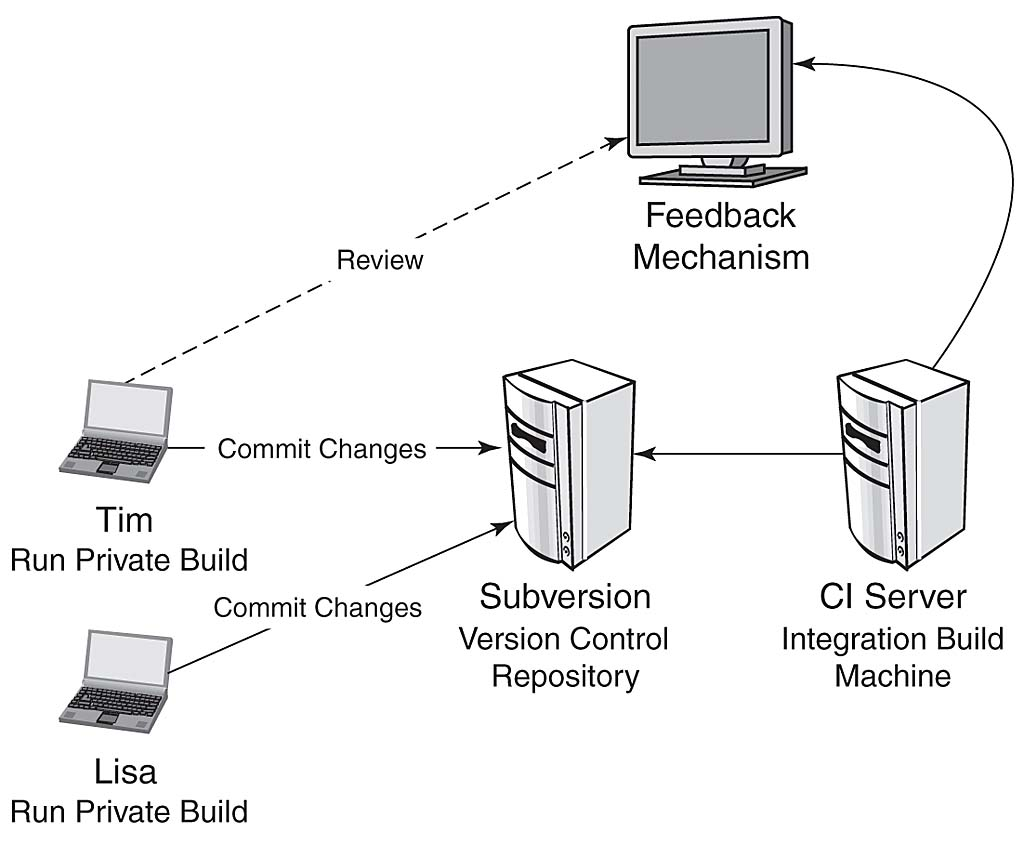
\includegraphics[width=0.6\linewidth,transparent]{images/ci.jpg}
  \end{center}

}


\frame{

  Continuous Integration

  \vspace{\baselineskip}

  \pause

  \begin{itemize}
    \item Automation!
    \item Use a source code repository
    \item Building \& deploying is automated
    \item Build is self-testing
    \item Commit frequently
    \item Build \& test every commit
    \item Test in a production clone
    \item Make it easy to get latest deliverables
    \item Hardcore: continuous deployment
  \end{itemize}

}


\frame{

  Continuous Integration tools

  \vspace{\baselineskip}

  {\small\begin{itemize}
    \item Subversion, Git, Mercurial, Bazaar, \ldots
    \item xUnit, Selenium, \ldots
    \item Make, Ant, Maven, \ldots
    \item Continuum, Gump, Bamboo, BuildBot, CruiseControl, Tinderbox,
    Jitterbug, \ldots
  \end{itemize}}

}


\frame{

  % http://www.flickr.com/photos/esti/4638056301/
  \begin{center}
    Pair Programming
    \vspace{\baselineskip}
    \vspace{\baselineskip}
    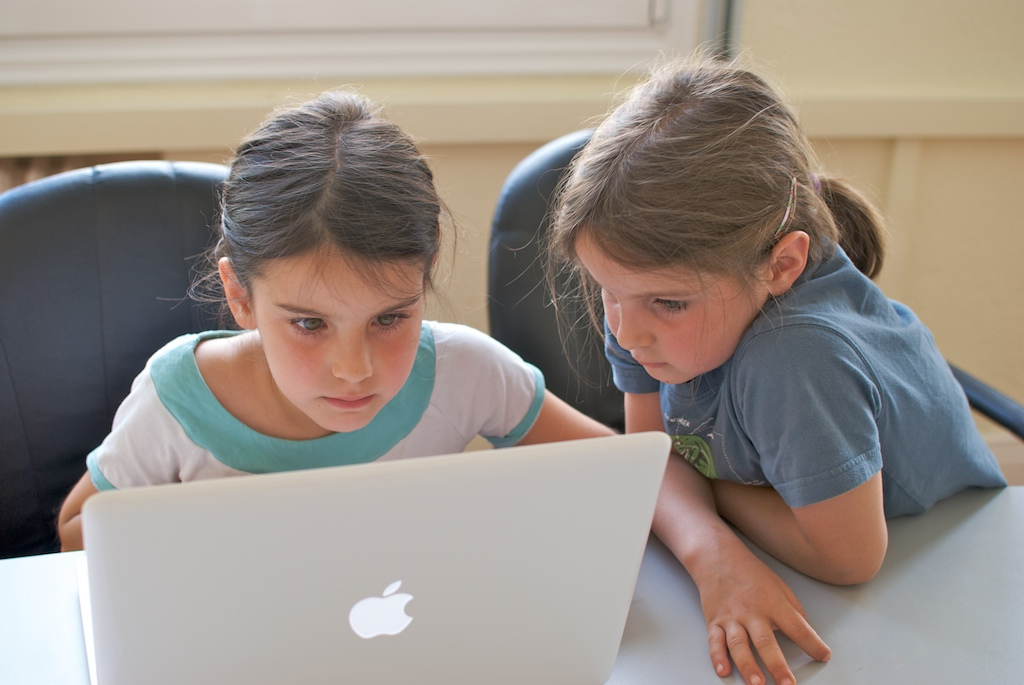
\includegraphics[width=0.8\linewidth,transparent]{images/pair-programming.jpg}
  \end{center}

}


\frame{

  Pair Programming

  \vspace{\baselineskip}

  \pause

  \begin{itemize}
    \item 2 programmers, 1 workstation
    \item {\bf driver} writes code
    \item {\bf observer}/navigator reviews
  \end{itemize}

  \vspace{\baselineskip}

  \pause

  Observer keeps high-level view, makes notes of likely problems.

  \vspace{\baselineskip}

  Driver is free to focus on a piece of code.

}


\frame{

  Variants of Pair Programming

  \vspace{\baselineskip}

  \pause

  {\em Ping pong pair programming}:
  {\small \begin{enumerate}
    \item observer writes failing unit test
    \item driver writes code to pass test
    \item repeat
  \end{enumerate}}

  \vspace{\baselineskip}

  \pause

  {\em Remote pair programming}\\
  {\small collaborative real-time editor, shared desktop (VNC), GNU screen in \texttt{-x} mode, IDE plugin, \ldots}

}


\frame{

  % http://www.flickr.com/photos/pulfi/3699253050/
  \begin{center}
    Sprints\\
    \vspace{\baselineskip}
    \vspace{\baselineskip}
    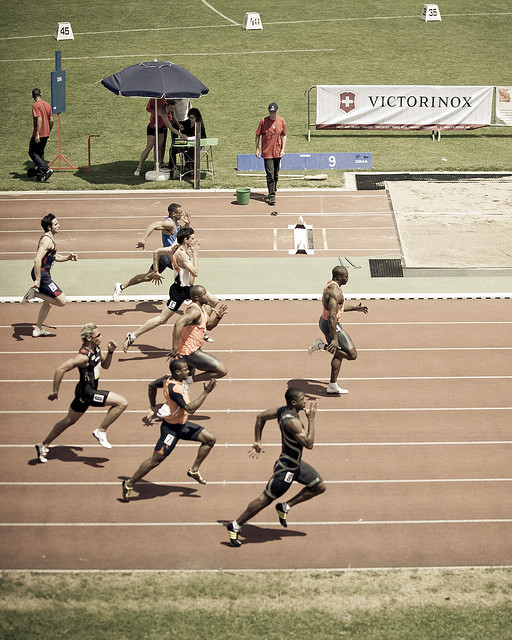
\includegraphics[height=0.6\paperheight,transparent]{images/sprint.jpg}
  \end{center}

}


\frame{

  Sprints

  \vspace{\baselineskip}

  \pause

  \begin{itemize}[<+->]
    \item short (1--2 days) intensive period of programming
    \item prepare a backlog of (yet unassigned) tasks
    \item one room
    \item small team (one coach)
    \item popularized in hackathons
  \end{itemize}

  \vspace{\baselineskip}

  \pause

  Also: scrum sprints

}


\frame{

  {\bf Discussion} -- {\em what methods do you use?}

  \vspace{\baselineskip}
  \vspace{\baselineskip}

  {\small
    m.vermaat.hg@lumc.nl

    \vspace{\baselineskip}
    \vspace{\baselineskip}

    %waterfall:
    \href{http://www.flickr.com/photos/hamed/462658709}{flickr.com/photos/hamed/462658709}\\
    %waterfall model:
    \href{http://www.flickr.com/photos/joomlatools/2283896218}{flickr.com/photos/joomlatools/2283896218}\\
    %thick-billed flowerpecker (dicaeum agile):
    \href{http://www.flickr.com/photos/snapflickr/3890553276}{flickr.com/photos/snapflickr/3890553276}\\
    %test tube:
    \href{http://www.flickr.com/photos/thebottomlesspaddlingpool/4767257252}{flickr.com/photos/thebottomlesspaddlingpool/4767257252}\\
    %paper party:
    \href{http://www.flickr.com/photos/carolnichols/2873491547}{flickr.com/photos/carolnichols/2873491547}\\
    %cat:
    \href{http://www.flickr.com/photos/paldies/85684217}{flickr.com/photos/paldies/85684217}\\
    %pair programming:
    \href{http://www.flickr.com/photos/esti/4638056301}{flickr.com/photos/esti/4638056301}\\
    %sprint:
    \href{http://www.flickr.com/photos/pulfi/3699253050}{flickr.com/photos/pulfi/3699253050}

    \vspace{\baselineskip}

    %continuous integration:
    \href{http://www.informit.com/title/0321336380}{Duvall, Matyas, and Glover. {\em Continuous Integration: Improving Software Quality and Reducing Risk}, 2007.}

  }

}


\end{document}
